\documentclass[a4paper,12pt]{article}

%%% Работа с русским языком
\usepackage{cmap}					% поиск в PDF
\usepackage{mathtext} 				% русские буквы в формулах
\usepackage[T2A]{fontenc}			% кодировка
\usepackage[utf8]{inputenc}			% кодировка исходного текста
\usepackage[english,russian]{babel}	% локализация и переносы
\usepackage{indentfirst}
\frenchspacing

\newcommand{\vyp}{\ensuremath{\hookrightarrow}}
\renewcommand{\epsilon}{\ensuremath{\varepsilon}}
\renewcommand{\phi}{\ensuremath{\varphi}}
\renewcommand{\kappa}{\ensuremath{\varkappa}}
\renewcommand{\le}{\ensuremath{\leqslant}}
\renewcommand{\leq}{\ensuremath{\leqslant}}
\renewcommand{\ge}{\ensuremath{\geqslant}}
\renewcommand{\geq}{\ensuremath{\geqslant}}
\renewcommand{\emptyset}{\varnothing}
\newcommand{\Ra}{\ensuremath{\Rightarrow}}
\newcommand{\ra}{\ensuremath{\rightarrow}}
\newcommand{\LRa}{\ensuremath{\Leftrightarrow}}
\newcommand{\tbf}{\textbf}
\newcommand{\ov}{\ensuremath{\overline}}
\newcommand{\CC}{\ensuremath{\mathbb{C}}}
\newcommand{\RR}{\ensuremath{\mathbb{R}}}
\newcommand{\NN}{\ensuremath{\mathbb{N}}}
\newcommand{\QQ}{\ensuremath{\mathbb{Q}}}
\newcommand{\ZZ}{\ensuremath{\mathbb{Z}}}

%%% Дополнительная работа с математикой
\usepackage{amsmath,amsfonts,amssymb,amsthm,mathtools} % AMS
\usepackage{icomma} % "Умная" запятая: $0,2$ --- число, $0, 2$ --- перечисление

%% Номера формул
%\mathtoolsset{showonlyrefs=true} % Показывать номера только у тех формул, на которые есть \eqref{} в тексте.
%\usepackage{leqno} % Нумереация формул слева

%% Свои команды
\DeclareMathOperator{\sgn}{\mathop{sgn}}

%% Перенос знаков в формулах (по Львовскому)
\newcommand*{\hm}[1]{#1\nobreak\discretionary{}
{\hbox{$\mathsurround=0pt #1$}}{}}



%%% Работа с картинками
\usepackage{graphicx}  % Для вставки рисунков
\graphicspath{{images/}{images2/}}  % папки с картинками
\setlength\fboxsep{3pt} % Отступ рамки \fbox{} от рисунка
\setlength\fboxrule{1pt} % Толщина линий рамки \fbox{}
\usepackage{wrapfig} % Обтекание рисунков текстом

%%% Работа с таблицами
\usepackage{array,tabularx,tabulary,booktabs} % Дополнительная работа с таблицами
\usepackage{longtable}  % Длинные таблицы
\usepackage{multirow} % Слияние строк в таблице

%%% Теоремы
\theoremstyle{plain} % Это стиль по умолчанию, его можно не переопределять.
\newtheorem{theorem}{Теорема}[section]
\newtheorem{proposition}[theorem]{Утверждение}
 
\theoremstyle{definition} % "Определение"
\newtheorem{corollary}{Следствие}[theorem]
\newtheorem{problem}{Задача}[section]
 
\theoremstyle{remark} % "Примечание"
\newtheorem*{nonum}{Решение}

%%% Программирование
\usepackage{etoolbox} % логические операторы

%%% Страница
\usepackage{extsizes} % Возможность сделать 14-й шрифт
\usepackage{geometry} % Простой способ задавать поля
	\geometry{top=20mm}
	\geometry{bottom=20mm}
	\geometry{left=5mm}
	\geometry{right=15mm}
 %
\usepackage{fancyhdr} % Колонтитулы
 	\pagestyle{fancy}
 	\renewcommand{\headrulewidth}{1pt}  % Толщина линейки, отчеркивающей верхний колонтитул
%\fancypagestyle{firstpage}{
	\rhead{\large{Исыпов Илья}}
%}
% 	\lfoot{Нижний левый}
% 	\rfoot{\large{Рябых Владислав, Б05-905}}
% 	\rhead{Верхний правый]}
% 	\chead{Верхний в центре}
 	\lhead{\large{Рябых Владислав}}
%	\cfoot{Нижний в центре} % По умолчанию здесь номер страницы

\usepackage{setspace} % Интерлиньяж
\onehalfspacing % Интерлиньяж 1.5
%\doublespacing % Интерлиньяж 2
%\singlespacing % Интерлиньяж 1

\usepackage{lastpage} % Узнать, сколько всего страниц в документе.

\usepackage{soul} % Модификаторы начертания

\usepackage{hyperref}
\usepackage[usenames,dvipsnames,svgnames,table,rgb]{xcolor}
\hypersetup{				% Гиперссылки
    unicode=true,           % русские буквы в раздела PDF
    pdftitle={Заголовок},   % Заголовок
    pdfauthor={Автор},      % Автор
    pdfsubject={Тема},      % Тема
    pdfcreator={Создатель}, % Создатель
    pdfproducer={Производитель}, % Производитель
    pdfkeywords={keyword1} {key2} {key3}, % Ключевые слова
    colorlinks=true,       	% false: ссылки в рамках; true: цветные ссылки
    linkcolor=red,          % внутренние ссылки
    citecolor=black,        % на библиографию
    filecolor=magenta,      % на файлы
    urlcolor=cyan           % на URL
}

\usepackage{csquotes} % Еще инструменты для ссылок

%\usepackage[style=authoryear,maxcitenames=2,backend=biber,sorting=nty]{biblatex}

\usepackage{multicol} % Несколько колонок

\usepackage{tikz} % Работа с графикой
\usepackage{pgfplots}
\usepackage{pgfplotstable}

\usepackage{caption}
\long\def\comment{}
\setlength{\abovecaptionskip}{7pt}
\setlength{\belowcaptionskip}{7pt}


\begin{document}
\author{Рябых Владислав и Исыпов Илья, Б05-905}
\title{\tbf{3.4.1.(4.13) Измерение магнитной восприимчивости диа- и парамагнетиков}}
\maketitle

\tbf{Цель работы:} измерение магнитной восприимчивости диа- и парамагнитного образцов.

\tbf{В работе используются:} электромагнит, аналитические весы, милливеберметр, источник питания постоянного тока, образцы диа- и парамагнетиков.


\section*{Теория}
копипаст из лабника/готового теха
используем формулу
\begin{equation}
	\text{что-то} = \dfrac{x}{y}
	\label{eq1}
\end{equation}

\section*{Экспериментальная установка}
(если она указана отдельно в лабнике/описании) также копипаст

\section*{Ход работы}
Делаем что-то по каким-то идеям. Рассчитываем что-то по формуле $\text{что-то} = \dfrac{x}{y}$, расчитываем погрешность как $\sigma_\text{что-то} = \text{что-то} \cdot \sqrt{\sigma_x^2 + \sigma_y^2}$. Результаты измерений приведены в таблице \ref{tab1}.

\begin{center}
\begin{tabular}{|c|c|c|c|c|c|c|c|c|c|}
	\hline
	$x$, A & 0.25 & 0.60 & 0.95 & 1.30 & 1.65 & 2.00 & 2.35 & 2.70 & 3.05 \\
	\hline
	$\Delta x$, А & 0.02 & 0.02 & 0.02 & 0.03 & 0.03 & 0.03 & 0.03 & 0.03 & 0.04 \\
	\hline
	$y$, мВб & 0.60 & 1.40 & 2.30 & 3.10 & 3.90 & 4.70 & 5.40 & 6.10 & 6.60 \\
	\hline
	$\Delta y$, мВб & 0.60 & 1.40 & 2.30 & 3.10 & 3.90 & 4.70 & 5.40 & 6.10 & 6.60 \\
	\hline
	$\text{что-то}$, Tл & 0.08 & 0.19 & 0.32 & 0.43 & 0.54 & 0.65 & 0.75 & 0.85 & 0.92 \\
	\hline
	$\Delta \text{что-то}$, Tл & 0.08 & 0.19 & 0.32 & 0.43 & 0.54 & 0.65 & 0.75 & 0.85 & 0.92 \\
	\hline
\end{tabular}
	\captionof{table}{градуировка электромагнита}\label{tab1}
\end{center}

Построим по данным из таблицы график зависимости $\text{что-то}(x)$, см. рис \ref{gr1}

\begin{center}
\begin{figure}[bhtp]
	\centering
	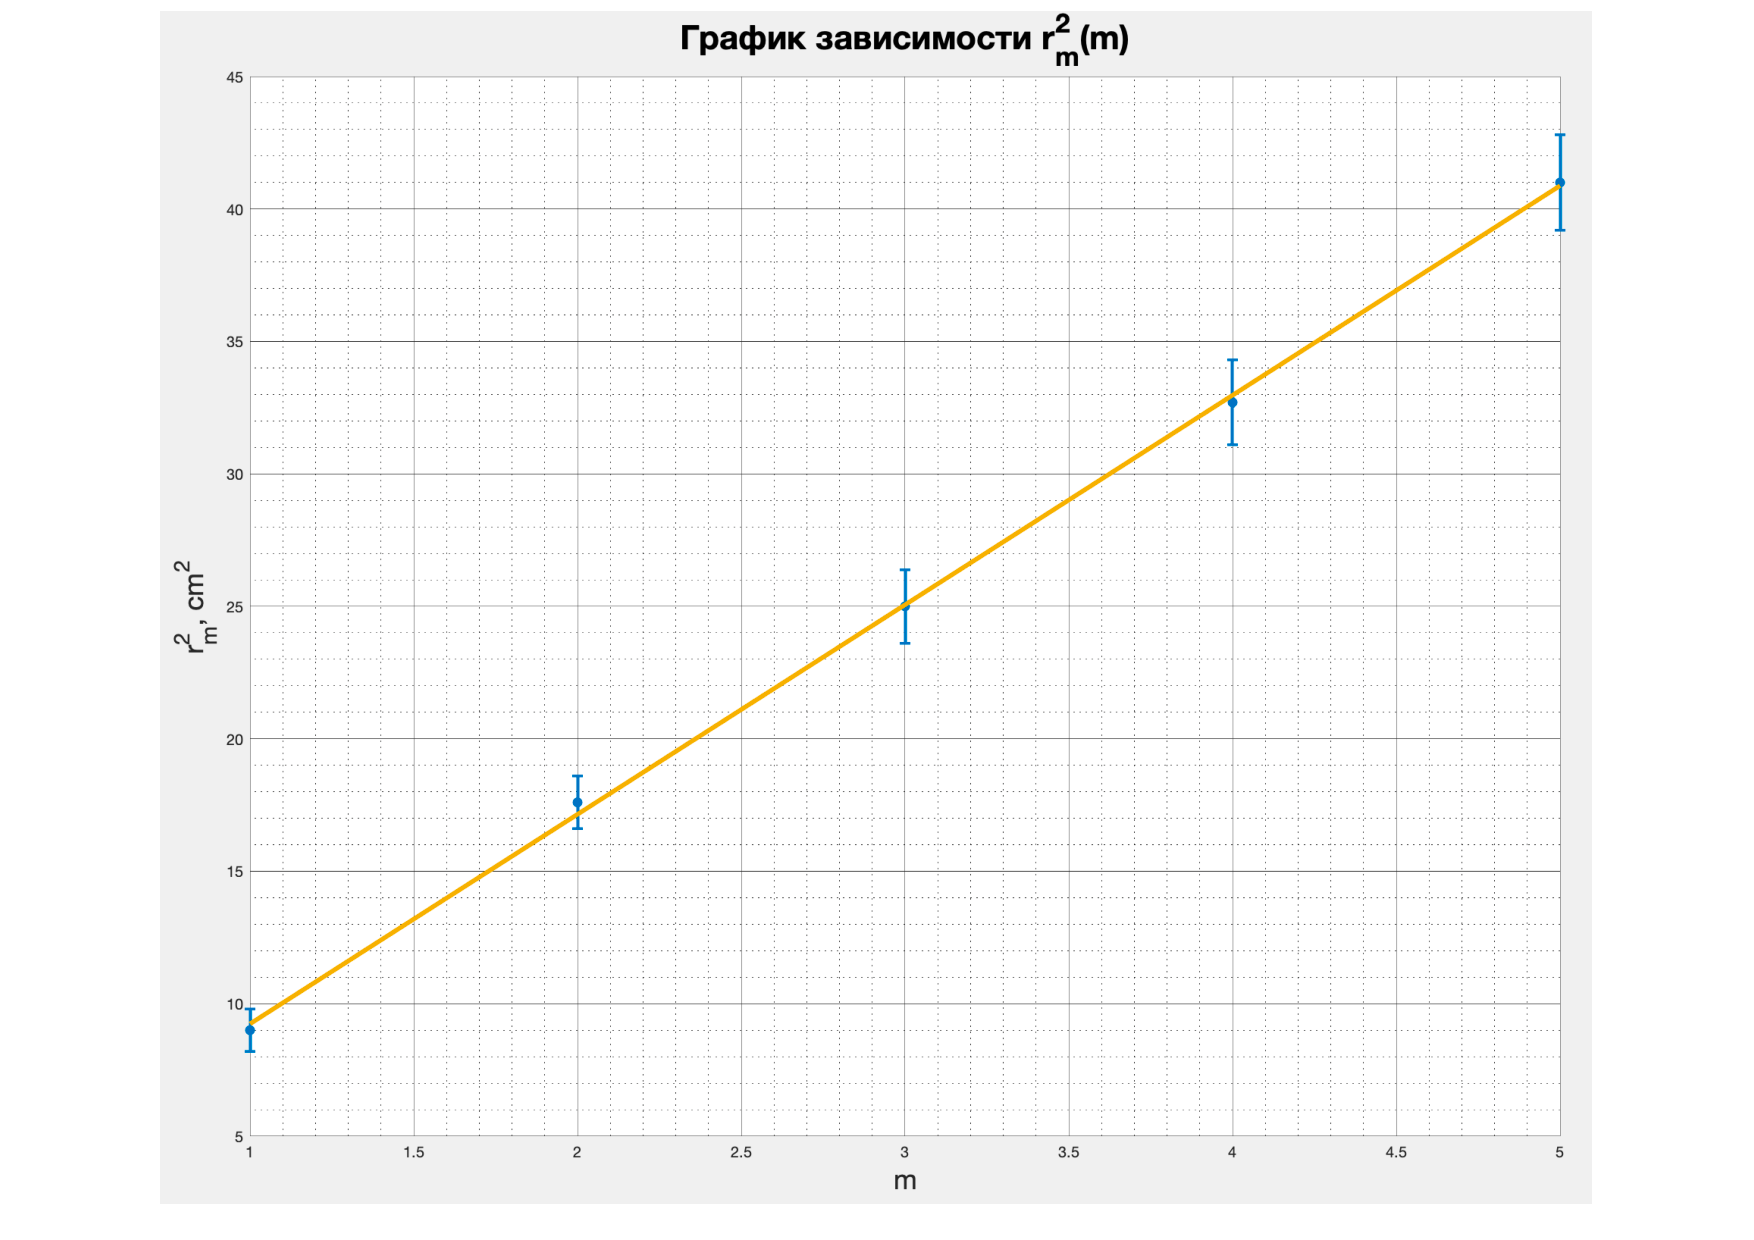
\includegraphics[width=\linewidth]{gr1.pdf}
	\caption{график зависимости $B(I)$}
	\label{gr1}
\end{figure}
\end{center}



По МНК находим, что: \[k_1 = (223 \pm 44)\dfrac{\text{мкН}}{\text{Тл}^2}, \ \ k_2 = (575 \pm 130)\dfrac{\text{мкН}}{\text{Тл}^2}\]


По формуле \eqref{eq1} рассчитаем что-то, погрешность рассчитываем по формуле:

Итого имеем
\[\text{что-то}_{\text{м}} = (-7.1 \pm 1.4) \cdot 10^{-6}, \ \  \text{что-то}_{\text{а}} = (18.4 \pm 4.2) \cdot 10^{-6}\]


(табличные значения для этих материалов: $\text{что-то}_{\text{м}} = -10.3 \cdot 10^{-6}, \ \  \text{что-то}_{\text{а}} = 23 \cdot 10^{-6}$)

\section*{Выводы}
\begin{enumerate}
	\item В ходе выполнения работы были расчитаны значения чего-то для меди и алюминия: $\text{что-то}_{\text{м}} = (-7.1 \pm 1.4) \cdot 10^{-6}, \  \text{что-то}_{\text{а}} = (18.4 \pm 4.2) \cdot 10^{-6}$, которые совпали с табличными значениями в пределах погрешности.
	\item Большая погрешность (20\% для меди и 23\% для алюминия) получилась вследствие больших неточностей в измерениях.
	\item Так как $\text{что-то}_{\text{м}} < 0$, а $\text{что-то}_{\text{а}} > 0$, можно сделать вывод, что медь -- это диамагнетик, а алюминий -- это парамагнетик.
\end{enumerate}


\end{document}